

\chapter{Latex Basics}
\label{chapter:basics}

\thispagestyle{empty}


Microsoft Word is not a good tool for writing books. Latex is a much
better tool. 
For those who have never used Latex before, I strongly recommend 
them to use Overleaf, which is an online LaTex editor that is easy to use,
and it is free. Installing LaTex software and all its package is not 
an easy job; using Overleaf, you don't need to install anything. 


\minitoc
\newpage



% *******************************************
% SECTION
% ******************************************* 
\section{Page Layout} 

The format of the book is defined here, including its trim size and 
margins. \texttt{7.5 x 9.25} is one of the standard trim sizes for 
textbooks. 
If you want to use a different trim size, you can adjust the
parameters. Do make sure that the trim size you choose is supported by the
self-publishing platform.  


\begin{lstlisting}
\documentclass[10pt]{book}

\usepackage{geometry}
\geometry{paperwidth=7.5in,paperheight=9.25in, bindingoffset=2cm,
          left=1.00in,right=0.50in,top=0.75in,bottom=0.50in,twoside}
\end{lstlisting}
 


% *******************************************
% SECTION
% *******************************************
\section{Abstract}
\label{basics:abstract}

For the first page of each chapter, the page number is printed in the footer, not
in the header. This will be out of bound when I submit it to KDP. 
A common practice is not to print out the page number for the first page.
That is why I set the style of this page to \texttt{empty}. 
I also use \texttt{minitoc} to include a mini table of content 
here. 

\begin{lstlisting}
\chapter{Basics}
\label{chapter:basics}

\thispagestyle{empty}

The abstract ...

\minitoc
\newpage
\end{lstlisting}



% *******************************************
% SECTION
% ******************************************* 
\section{Sections and Subsections} 

This part is the same as any typical paper. I do not have anything special
to say about it. Anybody who has used Latex to write papers before should have no problem with 
this part.




% *******************************************
% SECTION
% ******************************************* 
\section{Bibliography}

I use the \texttt{apalike} style for my bibliography. 
Please pay attention to the difference between \texttt{\textbackslash citep} and
\texttt{\textbackslash cite}. Here is an example using \texttt{\textbackslash citep}:  
Smith proposes a novel solution \citep{smith19}. 
Here is an example using \texttt{\textbackslash cite}: 
\cite{smith19} proposes a novel solution.

\begin{lstlisting}
\thispagestyle{empty}
\bibliographystyle{apalike}
\def\baselinestretch{1}
\bibliography{BibBook}
\end{lstlisting}

% *******************************************
% SECTION
% ******************************************* 
\section{Figures}

You can easily include a figure. 
Figure~\ref{fig:example} shows a figure example. 
The Latex code is shown below: 

\begin{figure}[htb]
\begin{center}
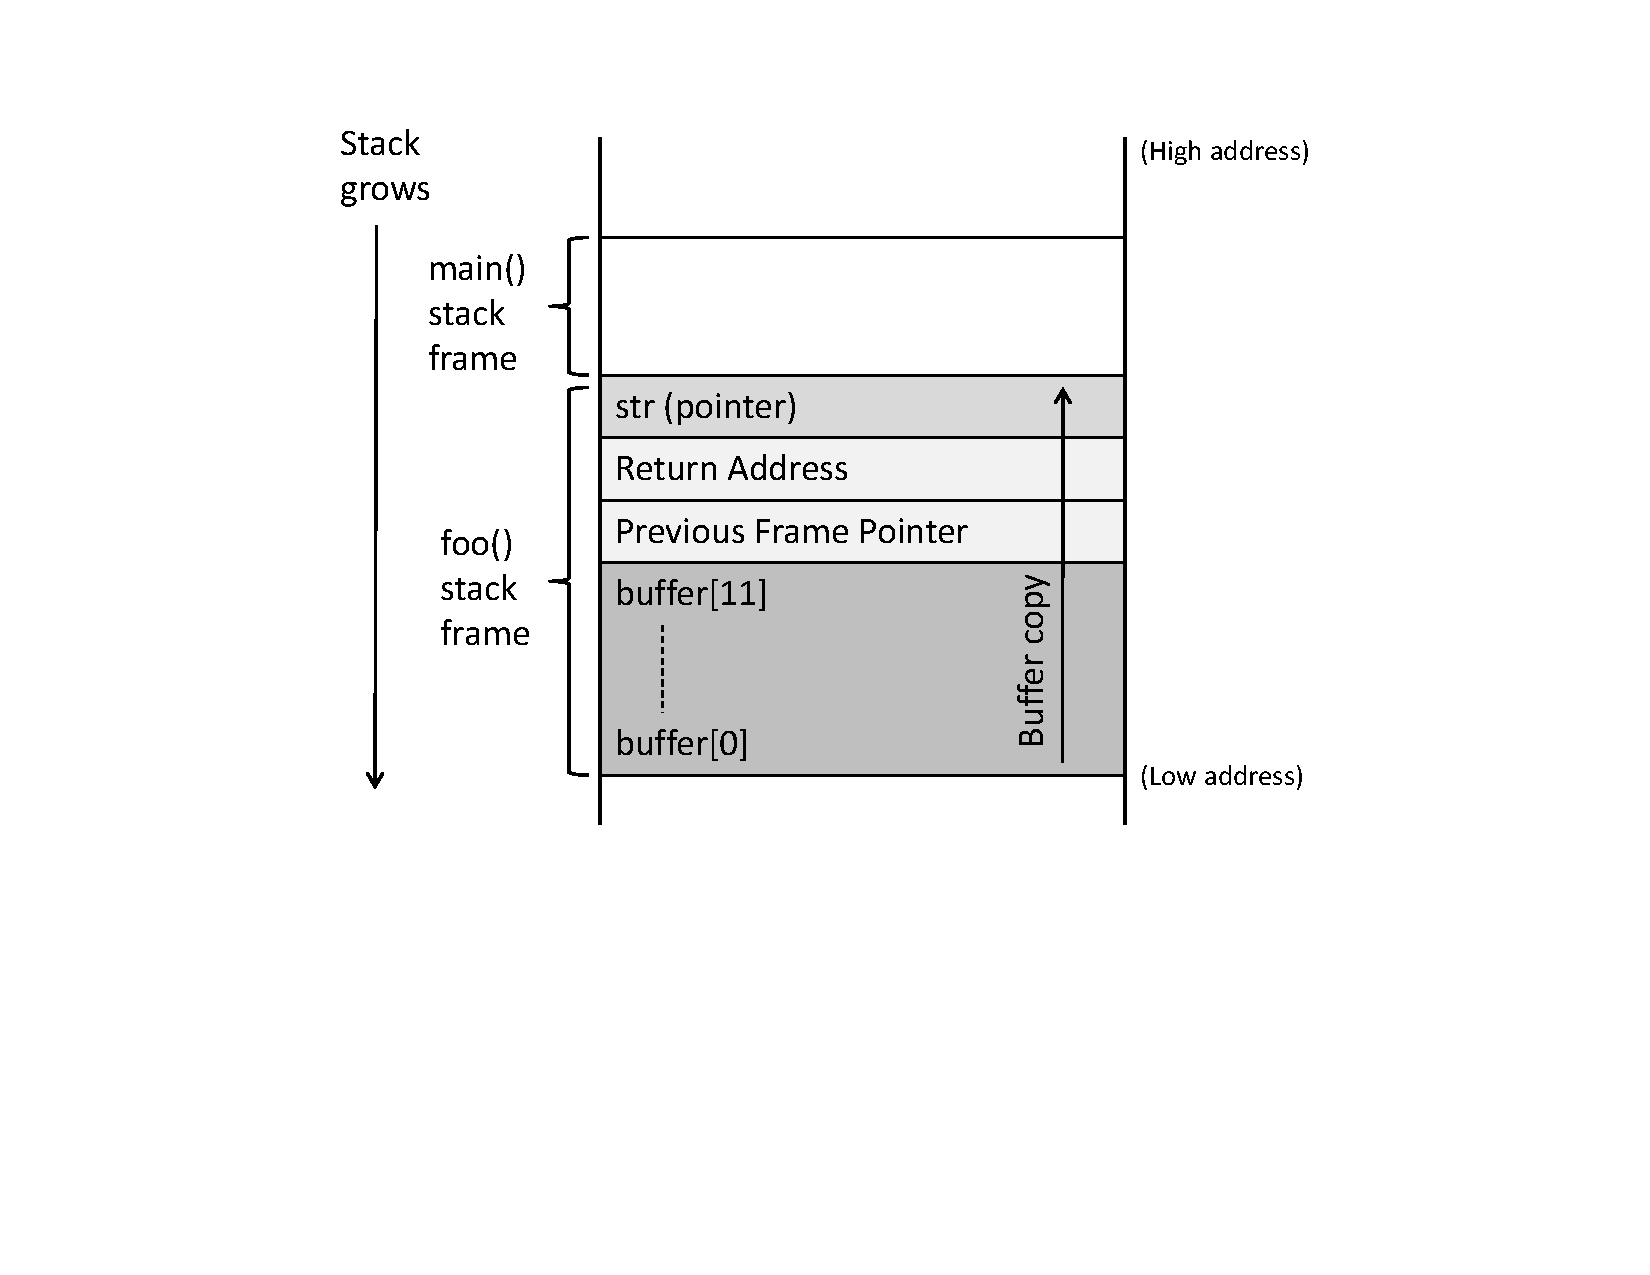
\includegraphics[width=0.8\textwidth]{./figure.pdf}
\end{center}
\caption{A figure example}
\label{fig:example}
\end{figure}
 



% *******************************************
% SECTION
% ******************************************* 
\section{Including Code}



\begin{lstlisting}[caption={The vulnerable program (\texttt{stack.c})},
                   label={buffer:stack_program}]
/* This program has a buffer overflow vulnerability. */
#include <stdlib.h>
#include <stdio.h>
#include <string.h>

int foo(char *str)
{
    char buffer[100];

    /* The following statement has a buffer overflow problem */
    strcpy(buffer, str);

    return 1;
}

int main(int argc, char **argv)
{
    char str[400];
    FILE *badfile;

    badfile = fopen("badfile", "r");        (*@\ding{192}@*)
    fread(str, sizeof(char), 300, badfile); (*@\ding{193}@*)
    foo(str);

    printf("Returned Properly\n");          (*@\ding{194}@*)
    return 1;
}
\end{lstlisting}
 

Sometimes, we need to refer to some particular lines in the code. I don't like to list 
the line numbers. Instead, I use the \texttt{ding} font to 
put a circled number in the lines that I would like to refer to. 
For example, I would say ``Line~\ding{192} opens a file ...''. 
This is much more convenient than referring to the actual line numbers. 
If you like another style of circled numbers, you can use
\ding{202}. \ding{203}, etc.






